\documentclass[12pt]{beamer}
\usetheme{Boadilla}
\usepackage{ragged2e}
\setbeamercovered{transparent}
\usepackage[utf8]{inputenc}
%\usepackage[brazil]{babel}
\usepackage{amsmath}
\usepackage{amsfonts}
\usepackage{mathtools}
\usepackage{amssymb}
\usepackage{graphicx}
\usepackage{tikz}
\usepackage{xypic}
\usepackage{seqsplit}
\usetikzlibrary{quotes,angles}
\usefonttheme{serif}
\author[]{Vinicius Martins Teodosio Rocha \\ Larissa Soares de Sousa
\\ Jose Jorge de Souza Silva}
\title[]{{\bf{Artimética com o \textit{Sagemath}}}}
\date{}
\institute[IFPB - CZ]{Instituto Federal da Paraíba - Campus Cajazeiras} 

\newcommand{\red}[1]{\color{red}#1\color{black}}
\newcommand{\blue}[1]{\color{blue}#1\color{black}}
\newcommand{\ils}[1]{\texttt{\color{black}{\colorbox{sageblue}{#1}}}}
\newcommand{\ilso}[1]{\texttt{\color{black}{\colorbox{lightgreen}{#1}}}}

\definecolor{sageblue}{HTML}{8BBEB2}
\definecolor{lightgreen}{HTML}{E6F9AF}%{1B264F}


\newcommand{\ZZ}{\mathbb{Z}}
\newcommand{\RR}{\mathbb{R}}
\newcommand{\FF}{\mathbb{F}}
\newcommand{\CC}{\mathbb{C}}
\newcommand{\QQ}{\mathbb{Q}}
\newcommand{\NN}{\mathbb{N}}
\newcommand{\PP}{\mathbb{P}}

\newcommand{\cA}{{\cal A}}
\newcommand{\cO}{{\cal O}}
\newcommand{\cE}{{\mathscr E}}
\newcommand{\cX}{{\cal X}}
\newcommand{\cT}{{\cal T}}
\newcommand{\cS}{{\cal S}}
\newcommand{\cK}{{\cal K}}
\newcommand{\cV}{{\cal V}}
\newcommand{\cW}{{\cal W}}


\newcommand{\ts}{\textsuperscript}

\newcommand{\supp}{{\rm Supp}}
\newcommand{\tsb}{\textsubscript}

\newcommand{\Pic}{\operatorname{Pic}}
\newcommand{\Spec}{\operatorname{Spec}}
\newcommand{\Proj}{\operatorname{Proj}}
\newcommand{\Div}{\operatorname{Div}}
\newcommand{\Tr}{\operatorname{Tr}}
\newcommand{\Gal}{\operatorname{Gal}}
\newcommand{\rk}{\operatorname{rk}}
\newcommand{\tors}{\operatorname{tors}}
\newcommand{\Sec}{\operatorname{Sec}}
\newcommand{\Id}{\operatorname{Id}}
\newcommand{\Het}{H_{\text{ét}}}
\newcommand{\rank}{\operatorname{rank}}
\newcommand{\Frob}{\operatorname{Frob}}
\newcommand{\res}{\operatorname{res}}
\newcommand{\Diff}{\operatorname{Diff}}
\newcommand{\NS}{\operatorname{NS}}
\newcommand{\Km}{\operatorname{Km}}
\newcommand{\Hom}{\operatorname{Hom}}
\newcommand{\End}{\operatorname{End}}
\newcommand{\MW}{\operatorname{MW}}
\newcommand{\mdc}{\operatorname{mdc}}
\newcommand{\sgn}{\operatorname{sgn}}
\newcommand{\legendre}[2]{\left(\frac{#1}{#2}\right)}


% especiais


\begin{document}
\begin{frame}
 \begin{figure}[t]
% \includegraphics[height=1.5cm]{cnpq.jpg}
% \hspace{5pt}
% \includegraphics[height=1.5cm]{logo_cnmac.png}
% \hspace{5pt}
 \includegraphics[width=\textwidth]{img/ecmat.png}
 \end{figure}
\titlepage
\end{frame}


\begin{frame}
  {O \textit{Sagemath}}
  \begin{itemize}
    \item \url{https://sagecell.sagemath.org/}
    \item Quase um Python com \textbf{muitas} ferramentas extras.
    \item Missão
    \begin{center}
      \textit{Criar uma alternativa viável de código aberto para o Magma,
      Maple, Mathematica e Matlab}
    \end{center}
    \item Licença GPL (GNU General Public License): Livre!
    \item \url{https://doc.sagemath.org/html/en/developer/}
    \item E o que tanto ele faz?
    \begin{itemize}
      \item \url{doc.sagemath.org/html/pt/tutorial/}
      \item \url{doc.sagemath.org/html/pt/a_tour_of_sage/}
      \item \url{doc.sagemath.org/html/en/thematic_tutorials/} só em inglês :(
    \end{itemize}
  \end{itemize}
\end{frame}


\begin{frame}
  {Gráficos}

  \begin{figure}[h]
    \centering
    \includegraphics[scale=0.4]{img/grafico01.png}
    \caption{Gráfico de $\sin(x), x \in [-\pi,\pi]$}
    \label{img:graficosin}
  \end{figure}

\end{frame}

\begin{frame}
  {Gráficos Interativos}
  \begin{figure}[h]
    \centering
    \includegraphics[scale=0.3]{img/grafico02.png}
    \caption{Gráfico de $x^n, x \in [-1,1]$, $n = 1,2,\dots$.}
    \label{img:graficoxn}
  \end{figure}
\end{frame}

\begin{frame}
  {Gráficos 3D}
  \begin{figure}[h]
    \centering
    \includegraphics[scale=0.3]{img/grafico03.png}
    \caption{Um parabolóide hiperbólico.}
    \label{img:graficoparab}
  \end{figure}
\end{frame}

\begin{frame}
  {Muitos gráficos juntos!}
  \begin{figure}[h]
    \centering
    \includegraphics[scale=0.4]{img/grafico04.png}
    \caption{Caminho poligonal sobre $y = sin(x)$.}
    \label{img:graficopolig}
  \end{figure}
\end{frame}

\begin{frame}
  {Cálculo Diferencial e Integral}
  \begin{figure}[h]
    \centering
    \includegraphics[scale=0.4]{img/calculo01.png}
    \caption{Derivadas e integrais}
    \label{img:derivint}
  \end{figure}
\end{frame}


\begin{frame}
  {Cálculo Diferencial e Integral}
  edos, series,?
\end{frame}


\begin{frame}
  {Matrizes}
  \begin{figure}[h]
    \centering
    \includegraphics[scale=0.4]{img/matrizes01.png}
    \caption{Manipulando matrizes}
    \label{img:manipmatriz}
  \end{figure}
\end{frame}

\begin{frame}
  {Álgebra Linear}
  \begin{figure}[h]
    \centering
    \includegraphics[scale=.4]{img/matrizes02.png}
    \caption{Polinômios, autovalores e decomposições}
    \label{img:alglin}
  \end{figure}
\end{frame}

\begin{frame}
  {Álgebra - Cálculo Simbólico}
  \begin{figure}[h]
    \centering
    \includegraphics[scale=.5]{img/algebra01.png}
    \caption{Manipulando expressões, resolvendo equações }
    \label{img:fatorando}
  \end{figure}
\end{frame}

\begin{frame}
  \begin{figure}[h]
    \centering
    \includegraphics[scale=0.4]{img/algebra02.png}
    \label{img:algebra02}
  \end{figure}
\end{frame}

\begin{frame}
  {Álgebra abstrata}
  \begin{figure}[h]
    \centering
    \includegraphics[scale=0.42]{img/abstrata01.png}
    \caption{Trabalhando com grupos}
    \label{img:abstrata01}
  \end{figure}
\end{frame}


\begin{frame}
{E muito mais:}
\begin{itemize}
  \item Combinatória, análise numérica, polinômios, grafos, etc
  \item Tópicos avançados (geometria algébrica, curvas elíticas, formas modulares, etc)
  \item Interface com outras ferramentas (GP/PARI, GAP, Singular,...)
  \item \LaTeX!
  \item Todo poder do \textit{Python}!
  \item O principal...
\end{itemize}
\end{frame}

\begin{frame}
\begin{center}
    {\Large Teoria dos Números}

    \vspace{0.8cm}
    
    \textit{A rainha da matemática}
  \end{center}
  \begin{figure}[h]
    \centering
    \includegraphics[scale=0.4]{img/gauss.jpeg}
    \caption{Carl F. Gauss}
    \label{img:label}
  \end{figure}
\end{frame}

\begin{frame}{Por quê?}
\justifying
\textit{``Associado ao pensamento computacional,
\textbf{cumpre salientar a
importância dos algoritmos e de seus fluxogramas}, que podem
ser objetos de estudo nas aulas de Matemática. Um algoritmo é
uma sequência finita de procedimentos que permite resolver um
determinado problema. [...] A linguagem algorítmica
tem pontos em comum com a linguagem algébrica, sobretudo em
relação ao conceito de variável. \textbf{Outra habilidade
relativa à álgebra que mantém estreita relação com o
pensamento computacional é a identificação de padrões
para se estabelecer generalizações, propriedades
e algoritmos.}}""
\begin{flushright}
  Brasil (2017). Base nacional comum curricular. Ministério da Educação e Cultura
\end{flushright}
\end{frame}


\begin{frame}
  {Computador não é o suficiente!}
  \pause
  $$
  \begin{array}{rl}
  31 & \text{ é primo }  \\ \pause
  331 & \text{ é primo }  \\ \pause
  3331 & \text{ é primo }  \\ \pause
  33331 & \text{ é primo }  \\ \pause
  333331 & \text{ é primo }  \\ \pause
  3333331 & \text{ é primo }  \\ \pause
  33333331 & \text{ é primo }  \\ \pause
  333333331 & \text{ é composto }  \\ \pause
  \end{array}
  $$
  $$
    333333331 = 17 \times 19607843
  $$
\end{frame}


\begin{frame}
  {Onde aprender?}
  \begin{itemize}
    \item Comput. Math. with SageMath
    \begin{itemize}
       \item  \url{http://sagebook.gforge.inria.fr/english.html}
     \end{itemize}
    \item Sage for undergraduates
    \begin{itemize}
      \item \url{people.vcu.edu/~clarson/bard-sage-for-undergraduates-2014.pdf}
    \end{itemize}
    \item Grátis (inglês/francês/alemão)
    \begin{figure}[h]
      \centering
      \begin{minipage}{.4\textwidth}
              \includegraphics[scale=0.15]{img/couverture_en.jpg}
      \caption{Comput. Math. with SageMath}
      \end{minipage}
      \begin{minipage}{.4\textwidth}
              \includegraphics[scale=0.2]{img/sfu.png}
      \caption{Sage for undergraduates}
      \end{minipage}
    \end{figure}
  \end{itemize}
\end{frame}
\begin{frame}
  {Em português}
\begin{minipage}{.5\textwidth}
  \begin{itemize}
    \item Elementos de comput. matemática com o Sagemath
    \begin{itemize}
      \item \url{https://loja.sbm.org.br/index.php/elementos-de-computac-o-matematica-com-sagemath.html}
    \end{itemize}
  \item Outros: \url{sagemath.org/library-publications.html\#books}
  \end{itemize}
\end{minipage}
\begin{minipage}{.4\textwidth}
    \begin{figure}[h]
    \centering
    \includegraphics[scale=0.3]{img/sbm.jpg}
  \end{figure}
\end{minipage}
\end{frame}

\begin{frame}
  {Como usar?}

\begin{itemize}
  \item Baixando e instalando.
  \begin{itemize}
    \item \url{www.sagemath.org/download.html}
    \item Windows, Mac e Linux
    \item \red{Não recomendável (pelo menos inicialmente)}
    \item Terminal e Jupyter
  \end{itemize}
  \item Cocalc
  \begin{itemize}
    \item \url{cocalc.com/}
    \item Colaborativo e interativo (mostro já!)
    \item Nuvem
  \end{itemize}
  \item SageMathCell
  \begin{itemize}
    \item \url{sagecell.sagemath.org/}
    \item \blue{Usaremos esse aqui!}
    \item Desvantagem: Não salva seu trabalho.
  \end{itemize}
\end{itemize}
\end{frame}


\section{Operações e Dados}
\begin{frame}
  {Tipos de dados $\dagger$}
  \begin{itemize}
    \item Números:
      \begin{itemize}
      \item Inteiros \ils{ZZ}
      \item Racionais \ils{QQ}
      \item Reais \ils{RR}
      \item Complexos \ils{CC}
      \end{itemize}
    \item Booleanos: Verdadeiro/Falso (True/False)
    \item Strings (textos!)
    \item $\rightarrow$ Listas $\leftarrow$
    \begin{itemize}
       \item Sequências indexadas por $0,1,2,\dots$
       \item \red{Não são exatamente conjuntos... mas servem}
       $$
       \{ x^2 \mid x \in \{1,\cdots, 5\}  \}
       $$
       \begin{center}
         \ils{[ x\^\,2 for x in [1..5]]}
       \end{center}
     \end{itemize} 
     \item Operações e funções
  \end{itemize}
\end{frame}

\begin{frame}
  {Finalmente...}
  \begin{block}
    {Teorema (Divisão euclidiana)} Sejam $a, b \in \ZZ$ com $b \neq 0$.
    Exitem $q, r \in \ZZ$ únicos tais que
    $$
      a = bq + r, r \in \{0,1,\dots,|b|-1\}
    $$
  \end{block}
  \begin{itemize}
    \item Método \ils{.quo\_rem()} (\textbf{Quo}tient e \textbf{Rem}ainder ---
    Quociente e resto)
    \item Uso: \ils{a.quo\_rem(b)}
    \item Retorna o par \ils{(q,r)}
    \item \red{Cuidado!}\ Para $b < 0$ o comportamento é diferente.
  \end{itemize}
\end{frame}

\begin{frame}
  {Divisores}
  \begin{itemize}
    \item Se o resto for zero dizemos
  que $b$ \emph{divide} $a$. A notação é $b \mid a$. 
    \item No sage isso se verifica com o método \ils{b.divides(a)}.
    \item Vamos criar uma lista com os divisores de $a$. $\dagger$
    \item \textbf{Desafio: } Um natural $n$ é \emph{perfeito} se é a
    soma de seus divisores próprios, e.g.
    $$6 = 1 + 2 + 3 \text{ e }28 = 1+2+4+7+14$$
    Encontre mais um número perfeito (Dica: Existe a função \ils{sum}!) \pause
    \item \textbf{Dever de casa 1}: Um teorema de Euclides/Euler classifica
        os perfeitos pares. Pesquise-o e encontre os 10 primeiros \pause
    \item \textbf{Dever(?) de casa 2}: Encontre um número perfeito ímpar.
  \end{itemize}
\end{frame}

\begin{frame}
  {Primos}
  \begin{itemize}
    \item Um natural $p > 1$ é primo seus divisores positivos são 
    $1$ e $p$.
    \item Como decidir se um dado $n$ é primo? \pause
    \item Testar se $n$ é divisível por algum inteiro $>1$ menor que ele. $\dagger$ \pause
    \item \textbf{Dever de casa}: Otimize o algoritmo acima.
    \item No sage: \ils{is\_prime()}
    \item Pseudoprimos.
    \item Outras funções envolvendo primos. $\dagger$
  \end{itemize}
\end{frame}

\begin{frame}
  {MDC}
  \begin{itemize}
    \item Maior divisor comum
    \item \ils{max([k for k in divisors(a) if k in divisors(b)])}
    \item Algoritmo de Euclides: \textbf{Lema:} $\mdc(a,b) = \mdc(b,a - kb)$
    \item $r$  resto da divisão de $a$ por $b \Rightarrow \mdc(a,b) = \mdc(b,r)$
    \item Divisões euclidianas sucessivas: $\dagger$
  \end{itemize}\vspace{-.5cm}
\begin{minipage}{0.5\textwidth}
  $$
  \begin{array}{rcrcc}
    \phantom{1001} &  & \phantom{9\times} \blue{a} &  & \red{b} \\[.2cm]
    1001 & = & 9\times \blue{109} & + & \red{20} \\[.2cm]
    {109} & = & 5 \times \blue{20} & + & \red{9} \\[.2cm]
    {20} & = & 2 \times \blue{9} & + & \red{2} \\[.2cm]
    9 & = & 4 \times \blue{2} & + & \red{1} \\[.2cm]
    2 & = & 2\times   \blue{1} & + & \red{0}.
  \end{array}
  $$
\end{minipage}
\begin{minipage}{0.4\textwidth}
    \vspace{0.8cm}
    $$
  \begin{array}{l}
    \rm{mdc}(1001,109) = \rm{mdc}(109,20) \\[.2cm]
    \rm{mdc}(109,20) = \rm{mdc}(20,9) \\[.2cm]
    \rm{mdc}(20,9) = \rm{mdc}(9,2) \\[.2cm]
    \rm{mdc}(9,2) = \rm{mdc}(2,1) \\[.2cm]
    \rm{mdc}(2,1) = \rm{mdc}(1,0) = 1 \\[.2cm]
  \end{array}
  $$
\end{minipage}
\end{frame}

\begin{frame}
  {Algoritmo de Euclides Estendido}
  \begin{itemize}
    \item \textbf{T. Bézout:} Existem $x,y \in \ZZ$ tais que
    $ax+by = \mdc(a,b)$. \pause
    \item As divisões sucessivas do Alg. de Euclides fornecem $x$ e $y$. \pause
    \item $\dagger$ Uma solução elegante: Seja $M = (m_{ij})\in \mathrm{M}_{3\times 2}(\ZZ)$,
    dada por 
   $$M 
   % = \begin{pmatrix}
   %    x_0 & x_1 \\
   %    y_0 & y_1 \\
   %    r_0 & r_1
   %  \end{pmatrix}
    = \begin{pmatrix}
      1 & 0 \\
      0 & 1 \\
      a & b
    \end{pmatrix}.
    $$
    Se $m_{32} \neq 0$, tome $q = \lfloor m_{31}/m_{32} \rfloor$ e substitua
  $$
    M \longleftarrow M 
    \begin{pmatrix}
      0 & 1 \\
      1 & -q
    \end{pmatrix}.
  $$
  Enquanto $m_{32} \neq 0$ repita esse processo. Quando $m_{32} = 0$ teremos
  que $m_{31} = \mdc(a,b)$ e $x = m_{11}$ e $y = m_{21}$ satisfazem 
  $ax+by = \mdc(a,b)$
  \end{itemize}

\end{frame}


\begin{frame}
  {Fatoração Única}
  \begin{block}
    {Teorema (Fundamental da Aritmética)} Todo inteiro $n>1$ pode ser
    escrito de forma única como produto de primos
    $$
      n = p_1p_2 \cdots p_k,
    $$
    com $p_1\leq p_2 \leq \cdots \leq p_k$.
  \end{block}
  \begin{itemize}
    \item Forma mais natural: Testar todos os primos! $\dagger$
    \item No sage: \ils{factor}
    \item Aplicação Importante: Criptografia!
  \end{itemize}
\end{frame}


\begin{frame}
  {Mini-Projeto: 1º dia}
  $$
    \frac{\#\{n \in \mathbb{N} \mid n \leq N \text{ e } p \mid n\}}
    {\#\{n \in \mathbb{N} \mid n \leq N\}}
      \to \frac{1}{p} \text{, quando $N \to \infty$}
  $$
  \begin{itemize}
    \item Prob. de um inteiro ser divisível por $p$ é $1/p$.
    \item Prob. de dois inteiros serem divisíveis por $p$ é
    $1/p^2$.
    \item Prob. de dois inteiros não serem simultaneamente divisíveis por $p$
    é $1 - \frac{1}{p^2}$
    \item Prob. de dois inteiros não serem simultaneamente divisíveis por 
    qualquer primo $p$ (i.e. serem coprimos!)
    $$
      \prod_{p \in P} \left(1 - \frac{1}{p^2}\right) = \cdots = \frac{6}{\pi^2}
    $$
    \item Tarefa: Escreva um código que dê aproximações para $\pi$ tomando
    pares de inteiros arbitrários e verificando se são coprimos.
  \end{itemize}
\end{frame}

\begin{frame}
  {Ideia:}
  \begin{itemize}
    \item Escolha um limite $K$ e uma quantidade de repetições $N$.
    \item Crie um contador $C$ para guardar os casos coprimos.
    \item Para $n = 1, \dots, N$
    \begin{itemize}
      \item Escolha $a,b$ aleatórios em $\{1, \dots, K\}$
      \item Se $\mdc(a,b) = 1$, aumente o valor no contador ($C \leftarrow C+1$)
    \end{itemize}
    \item Para $N$ e $K$ grandes devemos ter $\alpha:= C/N \approx 6/\pi^2$.
    \item Isole o $\pi$ na relação acima.
    \item Exiba uma aproximação para $\pi$ usando $\alpha$.
    \item Varie $K$ e $N$ e veja o efeito na aproximação.

  \end{itemize}
\end{frame}

\begin{frame}
  {Congruências}
  \begin{itemize}
    \item Pela divisão euclidiana, na divisão por $m>0$ há
    $m$ restos possíveis: $0, 1, \dots, m-1$,
    \item \textbf{Def.:} $a, b \in \ZZ$ são congruentes módulo $m$ se
    deixam o mesmo resto na divisão por $m$.
    \item Notação: $a \equiv b \pmod m$.
    \item Além do \ils{.quo\_rem()} há o operador \ils{\%}. $\dagger$
    \item Melhor ainda: \ils{mod}.
  \end{itemize}
\end{frame}

\begin{frame}
  \begin{itemize}
    \item Resumindo algumas aulas em poucos itens:
    \begin{itemize}
      \item A congruência respeita a aritmética.
      \item Na verdade, $\ZZ_m = \{0,1,\dots, m-1\}$
      com a relação de congruência é um anel $\rightarrow$ Resultado do
      \ils{mod}
    \end{itemize}
    \item É preferível trabalhar em $\ZZ_m$. 
    \begin{itemize}
      \item Manipulações mais complexas.
      \item Contas mais rápidas $\dagger$
    \end{itemize}
    \item Conexão com álgebra abstrata!
    \item Invertíveis.
    \item Função $\varphi$ de Euler.
  \end{itemize}
\end{frame}

\begin{frame}
  {Mini-Projeto 2º dia: Criptografia}

  A principal ferramenta matemática utilizada será o Teorema de Euler.

  \begin{theorem}
  [Teorema de Euler]
    Sejam $m\in \Bbb Z$ e $n>1$ natural com $m$ e $n$ coprimos.
    Então
    $$
      m^{\varphi(n)} \equiv 1 \pmod n,
    $$
    onde $\varphi$ é a função de Euler, definida por
    $$
      \varphi(n) =  \#\{ 1 \leq a \leq n \mid {\rm mdc}(a,n) = 1  \}
    $$
  \end{theorem}
\begin{itemize}
  \item  Recorde que em primos $p$, $\varphi(p) = p-1$.
  \item Além disso, $\varphi$ é multiplicativa, isto é, portanto
  se $p$ e $q$ são primos distintos então
  $$
    \varphi(pq) = \varphi(p)\varphi(q) = (p-1)(q-1)
  $$
\end{itemize}
\end{frame}

\begin{frame}
{\bf \large Criptografia assimétrica}
Ideia:
\begin{itemize}
  \item Sistema simétrico:
    \begin{itemize}
      \item Criptografar uma mensagem seria como colocar a mensagem numa caixa
       e fechar uma fechadura.
       \item Quem tem a chave da fechadura consegue abrir a caixa.
    \end{itemize}
  \item Sistema assimétrico:
    \begin{itemize}
      \item Fechadura especial com duas chaves: $k_p$ e $k_r$.
      \item Se a caixa é fechada com $k_p$, apenas é aberta com $k_r$.
      \item Se a caixa é fechada com $k_r$, apenas é aberta com $k_p$.
      \item {\bf Cada pessoa} tem um par $(k_p,k_r)$.
        \begin{itemize}
          \item $k_p$ é chamada de chave de pública.
          \item $k_r$ é chamada de chave de privada.
        \end{itemize}
      \item Formalmente $T_{k_p}^{-1} = T_{k_r}$, ou seja
      $$
        T_{k_r} ( T_{k_p}(m)) = m \text{ e } T_{k_p} ( T_{k_r}(m)) = m
      $$
    \end{itemize}
\end{itemize}
\end{frame}

\begin{frame}
  \begin{itemize}
    \item Todo mundo deixa a sua chave pública disponível.
    \item Por exemplo, se Alice deseja enviar uma mensagem para Bob, ela usa
    a chave publica de Bob $k_p^{(B)}$  (disponível para todos).

    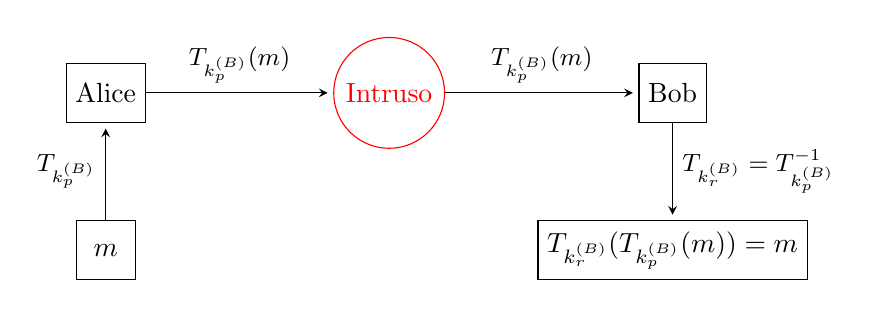
\begin{tikzpicture}[>=stealth,->,shorten >=2pt,looseness=.5,auto]
      \matrix [column sep={3.6cm,between origins},
      row sep={2cm,between origins},
      nodes={draw, minimum size=7.5mm}, ampersand replacement=\&]
      {
      \node (A) {Alice}; \& \node (I) [circle,red] {Intruso}; \& \node (B) {Bob}; \\
      \node (C) {$m$}; \& \& \node (D){$T_{k_r^{(B)}}(T_{k_p^{(B)}}(m)) = m$}; \\
      };
      \tikzstyle{every node}=[font=\small\itshape] 
      \draw (A) -- (I) node [midway] {$T_{k_p^{(B)}}(m)$};
      \draw (I) --  (B) node [midway] {$T_{k_p^{(B)}}(m)$};
      \draw (C) -- (A) node [midway] {$T_{k_p^{(B)}}$};
      \draw (B) -- (D) node [midway] {$T_{k_r^{(B)}} = T_{k_p^{(B)}}^{-1}$};
  \end{tikzpicture}
  \item A mensagem cifrada $T_{k_p^{(B)}}(m)$ só pode ser decifrada com a chave
  privada $T_{k_r^{(B)}}$ de Bob  (que só Bob tem)
  \item Vantagens:
  \begin{itemize}
    \item Não é necessário trocar chaves.
    \item Assinatura digital.
  \end{itemize}
  \end{itemize}
\end{frame}

\begin{frame}
  {O Algorítmo RSA (Encontrando um par de chaves)}
\begin{itemize}
  \item 
  \begin{itemize}
    \item Escolha primos $p$ e $q$ distintos
    \item Calcule $n = pq$
    \item Calcule $\varphi(n) = (p-1)(q-1)$
    \item Escolha $1 < e < \varphi(n)$ tal que ${\rm mdc}(e,\varphi(n)) = 1$.
    \item Calcule $d \equiv e^{-1} \pmod {\varphi(n)}$.
  \end{itemize}

  \item A chave publica consiste é o par $(n,e)$.
  \item A chave privada $k_r$ é o número $d$.
  \begin{itemize}
    \item Exceto pela chave publica, i.e., os números $n$ e $e$, todos os outros
    são guardados em segredo.
    \item Para encontrar $d$ a partir de $e$, é necessário  saber $\varphi(n)$
    \item Saber $\varphi(n)$ se resume a saber a fatoração de $n$.
    \item Se $p$ e $q$ forem primos muito grandes, encontrá-los a partir de $n$
    é uma tarefa muito dífícil.
  \end{itemize}
\end{itemize}
\end{frame}

\begin{frame}
  {\bf A cifragem}
  Nesse algorítmo, os textos são transformados em números inteiros $\mathrm{cod}$, com
  $0\leq \mathrm{cod} < n$.
  \begin{itemize}
    \item Suponha que, com o processo descrito acima, Bob tenha gerado sua
    chave pública $(n,e_B)$ e sua chave privada $d_B$.
    \item Alice, conhecendo $e_B$, cifra a mensagem $\mathrm{cod}$ via
    $$
      \mathrm{cod}_{\mathrm{cifrado}} = T_{k_p^{(B)}}(\mathrm{cod}) := \mathrm{cod}^{e_B} \pmod n
    $$
    \item Alice envia $c$ para Bob
    \item Bob decifra a mensagem $c$ via
    $$
      T_{k_r^{(B)}}(\mathrm{cod}_{\mathrm{cifrado}}) := \mathrm{cod}_{\mathrm{cifrado}}^{d_B} \equiv \mathrm{cod}^{e_Bd_B} \equiv \mathrm{cod} \pmod n
    $$
  \end{itemize}
  Pois $e_Bd_B \equiv 1 \pmod {\varphi(n)}$, logo $e_Bd_B  = q\varphi(n) + 1$
  
  Assim, pelo Teorema de Euler, $\mathrm{cod}^{\varphi(n)} \equiv 1 \pmod n$.
    $$
      \mathrm{cod}^{e_Bd_B} = \mathrm{cod}^{q\varphi(n) + 1}=
        (\mathrm{cod}^{\varphi(n)})^q\mathrm{cod} \equiv \mathrm{cod} \pmod n
    $$
\end{frame}

\begin{frame}
{\bf \large Observações:}
\begin{itemize}
  \item Os cálculos $\mathrm{cod}^{e_B} \pmod n$ e $c^{d_B} \pmod n$ são eficientes.
  \item Calcular $\phi(n)$ sem saber a fatoração de $n$, isto é $p$ e $q$,
  é difícil!
  \item Fatorar $n = pq$ é muito difícil.
  
    \begin{center}
      
    
    $n = RSA-240 = \seqsplit{12462036678171878406583504460810659043482037465167880575481878888328966680118821
          08550360395702725087475098647684384586210548655379702539305718912176843182863628 
          46948405301614416430468066875699415246993185704183030512549594371372159029236099}$ \pause
    \end{center}
    \begin{center}
    $p = \seqsplit{50943595228583991455505102358084371413264838202411147318666029652182120646974670
          0620316443478873837606252372049619334517}$
    \end{center}
    \begin{center}
     $q = \seqsplit{24462420883831815056781313902400289665380209257893140145204122133655847709517815
          5258218897735030590669041302045908071447}$
    \end{center}
    \begin{itemize}
      \item Fatorado em Novembro de 2019, usando supercomputadores.
      \item $\sim$ 900 cores-anos
  \end{itemize}
\end{itemize}
\end{frame}



\begin{frame}
  {Sistemas de congruências}
\begin{block}
  {Teorema} Se $m_1$ e $m_2$ são coprimos
  $$
  \begin{cases}
    x \equiv a_1 \pmod{m_1} \\
    x \equiv a_2 \pmod{m_2} \\
  \end{cases}
  $$
  tem solução única módulo $m_1m_2$.
\end{block}
\begin{itemize}
  \item Solução: $x = a_1 m_2 m_1' + a_2 m_1 m_2'$
onde $m_1'$ é o inverso de $m_2$ módulo $m_1$ e $m_2'$
é o inverso de $m_1$ módulo $m_2$.
  \item \red{Atenção:}\ Não podemos misturar os módulos
  \begin{itemize}
    \item Usar \ils{inverse\_mod}
  \end{itemize}
  \item No sage: \ils{crt}
\end{itemize}
\end{frame}



\begin{frame}
  {Ideias de projetos}
  \begin{itemize}
    \item Equações diofantinas
    \begin{itemize}
      \item Força bruta / otimizações
      \item Soluções parametrizáveis (ternos pitagóricos, Pell, etc.)
      \item Inexistência de soluções via redução módulo $m$.
    \end{itemize}
    \item Criptografia: RSA, Diffie-Hellman, $M_n(\ZZ_m)$, etc
    \item Códigos
  \end{itemize}
\end{frame}

\begin{frame}
  {Outras Referências / Links }
  \begin{itemize}
    \item Livros online
    \begin{itemize}
      \item Teoria dos Números \url{http://math.gordon.edu/ntic/}
      \item Álgebra abstrata \url{http://abstract.ups.edu/aata/aata.html}
    \end{itemize}
    \item \url{https://www.sagemath.org/library.html}
    \item \url{https://www.sagemath.org/library-publications.html}
    \item Euler project (\url{https://projecteuler.net/})
  \end{itemize}
\end{frame}
\end{document}

